%=================================================
% Economics Coursework Template (Beamer)
%=================================================
\documentclass[10pt]{beamer}

\usetheme{default}
\usecolortheme{default}
%------------ Packages ------------
\usepackage{lmodern}
\usepackage{amsmath, amssymb}
\usepackage{booktabs}
\usepackage{graphicx}
\usepackage{natbib}
\usepackage[hidelinks]{hyperref}
\usepackage{xcolor}
\usepackage[dvipsnames]{xcolor}
\usepackage{tikz}
\usepackage{svg}
\usepackage{subcaption}

%------------ Title ------------
\title{\Large Detection of Oil \& Gas Activity Using Satellite Data in Southern Kurdistan}
\author{\scriptsize Nardeen Abdulkareem - The University of Toronto \\ 
        \texttt{nardeen.abdulkareem@mail.utoronto.ca} \\ 
        \today}
\date{\vspace{-15mm}}

%------------ Begin Document ------------
\begin{document}

% Title slide
\begin{frame}
  \vspace{1.2cm}
  \titlepage
\end{frame}
\begin{frame}{Motivation}
Reliable measurement of economic activity such as gross domestic product in developing
countries is a persistent challenge facing economists. Many developing nations lack the capacity to operate a competent statistical agency. Even developed countries such as China are often accused of falsifying or withholding information regarding the country's economic activity. \\\


Advancements in machine learning models allow the research to reduce the amount of asymmetry in information related to the availability of data. Specifically, Yang, Ai, and Arkolakis (2025) have greatly inspired the choice of variables, implementation, and analysis that follows.
\end{frame}

\begin{frame}{Objective}
This research is focused on developing a consistent, high quality framework for the measurement of economic activity of the oil and gas sector in Southern Kurdistan using satellite data on night time lights, heat signatures, land temperatures, and pollution. \\\ 


Once we have constructed our dataset, we use our results to measure outcomes regarding economic activity across space. Satellite variables serve as noisy but informative proxies for latent economic output at fine geographic resolution. 
\end{frame}

\begin{frame}{Economic Contribution}
\begin{itemize}
\item Provides high-frequency, spatially granular measurement of oil and gas activity in data-scarce regions
\item Enables real-time monitoring of production in politically unstable environments
\item Allows estimation of:
\begin{itemize}
\item Regional output and growth
\item Informal or unreported extraction activity
\item Effects of conflict and sanctions on energy supply
\end{itemize}
\item Bridges remote sensing with applied economic measurement
\end{itemize}
\end{frame}

\begin{frame}{Raw Data}

\begin{figure}
\centering
\begin{subfigure}{0.49\textwidth}
    
\includegraphics[width=\linewidth]{0.png}
\end{subfigure}
\hfill
\begin{subfigure}{0.49\textwidth}
    
\includegraphics[width=\linewidth]{2.png}
\end{subfigure}

\end{figure}

\end{frame}

\begin{frame}{Data}
\textbf{Gas Flaring Data (NASA): VIIRS Nightfire / VNF (NASA)} 
\begin{itemize} 
\item Daily global detection of gas flaring activity 
\item Captures natural gas combustion, or flare location
\item Used to train ML model 
\item \textbf{Time Coverage:} 2012 -- 2024. Aggregated to monthly grid level 
\end{itemize}
\vspace{0.2cm}
\textbf{Sentinel-2 (ESA)} 
\begin{itemize} 
\item Optical bands (10–20m resolution) 
\item Surface reflectance (NDVI, NDBI inputs) 
\item Coverage: 2017 -- 2024 
\end{itemize}

\end{frame}

\begin{frame}{Data}
\textbf{VIIRS Nighttime Lights (NOAA)} 
\begin{itemize} 
\item Nighttime luminosity (industrial activity and growth proxy) 
\item Coverage: 2012 -- 2024 
\end{itemize} 
\vspace{0.2cm} 
\textbf{Land Surface Temperature (MODIS)} 
\begin{itemize} 
\item Nighttime thermal emissions 
\item Coverage: 2012 -- 2024 
\end{itemize} 
\vspace{0.2cm} 

\textbf{Spatial and Temporal Structure} 
\begin{itemize} 
\item Study region: Southern Kurdistan (Iraqi Jurisdiction) 
\item Grid: 1 km $\times$ 1 km cells 
\item Panel dataset: Grid $\times$ Month 
\end{itemize}
\end{frame}


\begin{frame}{Feature Space}
\textbf{Spectral Features}
\begin{itemize}
    \item Sentinel-2 surface reflectance bands:
    \begin{itemize}
        \item B4 (Red)
        \item B8 (Near Infra-red)
        \item B11 (Short-Wave Infra-red)
    \end{itemize}
    \item Vegetation and land-use indices:
    \begin{itemize}
        \item NDVI (Vegetation Index)
        \item NDBI (Built-up Index)
        \item Built-up index (A constructed relative index $NDBI_{it} - NDVI_{it}$)
    \end{itemize}
    \item Gas flaring and industrial heat emissions produce strong signals in the
short wave infra-red band relative to near-infra-red signals. 
    \begin{itemize}
        \item NIR / Red
        \item SWIR / NIR % Elevated SWIR-to-NIR ratios are indicative of thermal emissions and combustion activity associated with flaring:
        \item SWIR / Red
    \end{itemize}
\end{itemize}


\end{frame}

\begin{frame}{Feature Space}
\textbf{Temporal Features}
\begin{itemize}
    \item Rolling averages: 3-month and 6-month windows to capture persistence
    \item Monthly first differences: night lights, surface temperature, and SWIR to capture persistence
    \item Anomaly measures: deviations from local average in spectral variables.
\end{itemize}

\textbf{Naive Constructed Oil \& Gas Signals}
\[
\text{OilSignature}_{it}
=
\text{NTL}_{it}
+
\text{BuiltupIndex}_{it}
+
\text{SWIRNIRRatio}_{it}
+
\text{LST}_{it}
-
\text{NDVI}_{it}
\]
\vspace{0.2cm} 

\textit{Seasonal control are used to capture patterns in vegetation, temperature, and illumination over time. As well as interaction terms to capture joint effects.}
\end{frame}

\begin{frame}{Machine Learning Model}
\[
\hat p_{it} = \Pr(Y_{it}=1 \mid X_{it})
\]
where \(Y_{it}\) indicates known flaring and \(X_{it}\) contains our features.

\vspace{0.6em}

\textbf{Model}

\vspace{0.3em}

\begin{itemize}
\item Histogram-based Gradient Boosting classifier
\item Trained on pre-2023 data, tested on post-2023 data
\item We handle missing data via median imputation and indicators
\item Addresses class imbalance via weighted loss
\end{itemize}

\textbf{Estimation}
\[
\min_f \sum_{i,t} w_{it}
\left[
- Y_{it}\log \hat p_{it}
- (1-Y_{it})\log(1-\hat p_{it})
\right]
\]

\textbf{Output}
\begin{itemize}
\item \(\hat p_{it} \in [0,1]\): flare-like probability score
\item High probability grids identified via a threshold and persistence over time
\end{itemize}
\end{frame}

\begin{frame}{Model Diagnostics}
\begin{figure}
\centering
\begin{subfigure}{0.49\textwidth}
    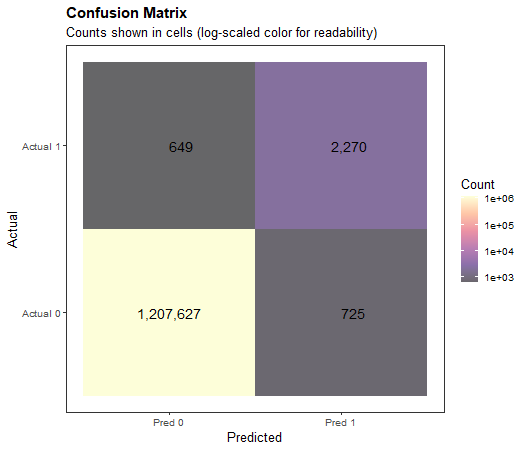
\includegraphics[width=\linewidth]{9.png}
\end{subfigure}
\hfill
\begin{subfigure}{0.49\textwidth}
    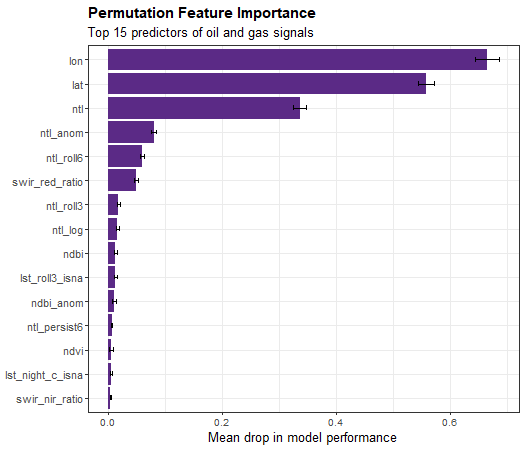
\includegraphics[width=\linewidth]{10.png}
\end{subfigure}

\end{figure}

\end{frame}


\begin{frame}{Model Efficiency}
\begin{itemize}
\item ROC-AUC = 0.999 (Measures ranking ability to be nearly perfect)
\item PR-AUC = 0.841 (Measures accuracy for rare events. The model remains highly precise as detection increases)
\end{itemize}

\vspace{0.2cm} 

\textbf{Threshold}
\begin{itemize}
\item Optimal threshold: \(\tau = 0.977\)
\item Selected to maximize F1-score (0.768)
\end{itemize}

\vspace{0.2cm} 

\textbf{Interpretation}
\begin{itemize}
\item The model is extremely good at \textbf{ranking locations by risk}
\item Because true sites are rare, we use a \textbf{high threshold} to avoid false detections
\item Only locations with \textbf{very strong signals} are classified as oil/gas candidates
\end{itemize}
\end{frame}

\begin{frame}{Predicted Sites For Oil and Gas Activity}
\begin{figure}
\centering
\begin{subfigure}{0.49\textwidth}
    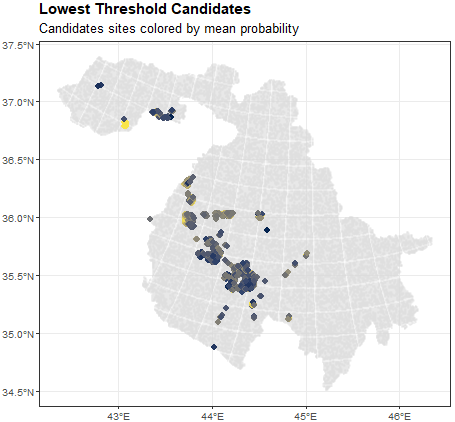
\includegraphics[width=\linewidth]{8.png}
\end{subfigure}
\hfill
\begin{subfigure}{0.49\textwidth}
    
\includegraphics[width=\linewidth]{7.png}
\end{subfigure}

\end{figure}
\end{frame}

\begin{frame}{Empirical Question: Are Detected Signals Persistent?}
Machine learning helps us identify the locations of oil and gas activity. But you may ask yourself are these signals just noise? Do high probability locations exhibit \textbf{persistent activity over time}?

\vspace{0.8em}

\textbf{Approach}

\vspace{0.4em}

\begin{itemize}
\item Construct a panel of grid cells at monthly frequency
\item Define a high activity indicator (the top 5\% of predicted probabilities)
\item Test whether high activity status today predicts future high activity
\end{itemize}

\vspace{0.8em}

\textbf{Reasoning}

\vspace{0.4em}

\begin{itemize}
\item Oil and gas sites are \textbf{persistent} (due to fixed and expensive infrastructure)
\item Random noise would yield \textbf{sporadic and short lived results}
\end{itemize}
\end{frame}

\begin{frame}{Regression Results}
\[
\text{HighRisk}_{it}
= \sum_{k=1}^{3} \beta_k \,\text{HighRisk}_{i,t-k}
+ \alpha_i + \gamma_m + \varepsilon_{it}
\]
\centering
\resizebox{\textwidth}{!}{
\begin{tabular}{lcccccc}
   \tabularnewline \midrule \midrule
   Dependent Variable: & \multicolumn{6}{c}{95 Percentile of Probability of Activity}\\
                   & OLS            & Month FE       & Grid FE        & Grid + Month FE & 2 Lags         & 3 Lags \\   
   Model:          & (1)            & (2)            & (3)            & (4)             & (5)            & (6)\\  
   \midrule
   \emph{Variables}\\
   Constant        & 0.0229$^{***}$ &                &                &                 &                &   \\   
                   & (0.0032)       &                &                &                 &                &   \\   
   High-prob (t-1) & 0.4851$^{***}$ & 0.4844$^{***}$ & 0.3011$^{***}$ & 0.2964$^{***}$  & 0.2759$^{***}$ & 0.2775$^{***}$\\   
                   & (0.0237)       & (0.0238)       & (0.0236)       & (0.0234)        & (0.0260)       & (0.0267)\\   
   High-prob (t-2) &                &                &                &                 & 0.0163         & 0.0095\\   
                   &                &                &                &                 & (0.0167)       & (0.0177)\\   
   High-prob (t-3) &                &                &                &                 &                & 0.0049\\   
                   &                &                &                &                 &                & (0.0144)\\   
   Grid FE         & No             & No             & Yes            & Yes             & Yes            & Yes\\  
   Month FE        & No             & Yes            & No             & Yes             & Yes            & Yes\\  
   \midrule
   Observations    & 18,605         & 18,605         & 18,605         & 18,605          & 18,330         & 18,055\\  
   R$^2$           & 0.24904        & 0.25666        & 0.34478        & 0.35320         & 0.34348        & 0.34621\\  
   Adjusted R$^2$  & 0.24900        & 0.25618        & 0.33495        & 0.34310         & 0.33303        & 0.33561\\  
   Within R$^2$    &                & 0.24772        & 0.09609        & 0.09282         & 0.08206        & 0.08058\\  
   \midrule \midrule
   \multicolumn{7}{l}{\emph{Clustered standard-errors in parentheses}}\\
   \multicolumn{7}{l}{\emph{Signif. Codes: ***: 0.01, **: 0.05, *: 0.1}}\\
\end{tabular}
}
\end{frame}


\begin{frame}{Limitation} 
\textbf{Limitations}
\begin{itemize}
\item \textbf{Temporal uncertainty:} Satellite observations are discrete and noisy, making it difficult to fully characterize continuous activity dynamics over time
\item \textbf{Limited classification:} The model detects activity, but does not distinguish between different facility types (e.g., oil wells vs. refineries)
\item \textbf{Measurement error:} Remote sensing data are subject to noise, missing values, and environmental interference, which may affect prediction accuracy
\item \textbf{Ordinal Measurements:} We have yet to estimate the amount extracted or refined at these facility.
\end{itemize}

\end{frame}

\begin{frame}{Next Steps}
\textbf{Next Step}
\begin{itemize}
\item \textbf{Neural networks:} Incorporate computer vision to distinguish between different facility types
\item \textbf{Price elasticity:} Link detected activity to global oil prices to estimate supply responsiveness
\item \textbf{Policy analysis:} Empirically evaluate the impact of sanctions on Iran and regional conflict on oil and gas activity in Kurdistan
\end{itemize}
\end{frame}

\begin{frame}{Temporal Patterns}
\begin{figure}
\centering

    
\includegraphics[width=\linewidth]{6.png}


\end{figure}
\end{frame}

\end{document}




